\textit{You Only Look Once: Unified, Real-time Object Detection}(YOLO)\cite{yolo}是单阶段检测方法的开山之作。正如其名:“你只需要看一次”,它只处理一次图片即可同时得到目标的位置和其属于什么类别,将目标检测任务描述为一个端到端、统一的回归问题。“One Stage”最核心的思想可以概括为:首先对全图给出一个大概的范围进行分类,利用了分类器优秀的分类效果,不断迭代直到得出一个精细的位置,
\begin{uscfigure}
	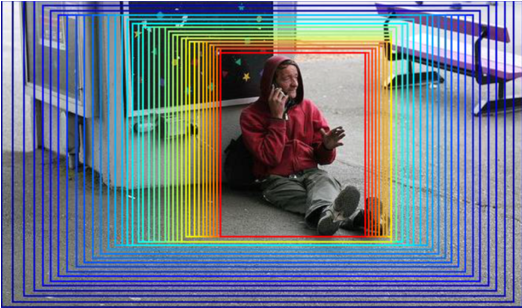
\includegraphics[width=\textwidth]{./Pictures/od_regressor.png}	
	\caption{YOLO}
	\label{yolo}
\end{uscfigure}
“One Stage”回归的思想如图\ref{yolo}从蓝色的框框到红色的框框,这样的检测速度一定很快,但是对小尺度目标的检测也肯定不好。

\subsubsection{YOLO}
\textbf{YOLO}是“One Stage”方法中的典型算法。首先将原始图片调整到一个固定尺寸,再将调整后的图片划分成一个SxS的网格,每个网格负责检测该网格区域内的物体的类别和位置。

更具体的是如下定义:
\begin{equation}
	Pr(Class_i | Object) * Pr(Object) * IOU_{pred}^{truth} = Pr(Class_i) * IOU_{pred}^{truth}
\end{equation}
YOLO算法基于分而治之的策略,将从卷积后的原始图片中提取到的特征图分为SxS块,然后对每一块进行分类,并使用非极大值抑制(NMS\cite{soft-nms})算法去除重叠的框,最终得到想要的结果。
\subsubsection{SSD}
YOLO检测速度非常快,但是问题就在于该算法对小物体的检测效果不好。为解决这个问题,SSD就在YOLO的想法上融合了Faster R-CNN的Anchor概念,并在不同尺度的卷积层的特征图上做出预测。关于SSD算法的细节介绍将在第三章将详细阐述。
